\documentclass[11pt]{article}
\usepackage[margin=1in]{geometry}
\usepackage{amsmath,amssymb,bm}
\usepackage[T1]{fontenc}
\usepackage[utf8]{inputenc}
\usepackage{lmodern}
\usepackage{booktabs}
\usepackage{array}
\usepackage{enumitem}
\usepackage{hyperref}
\usepackage{tikz}
\usetikzlibrary{arrows.meta,positioning,calc,fit,shapes.geometric}

\title{Roll and Pitch Observability in a Local IMU/GNSS EKF}
\author{sensor\_fusion documentation}
\date{\today}

\newcommand{\T}{^{T}}
\newcommand{\dt}{\Delta t}
\newcommand{\phiv}{\delta\phi_v}
\newcommand{\rhom}{\delta\rho_b}
\newcommand{\thetav}{\delta\theta_v}
\newcommand{\pim}{\delta\pi_b}

\begin{document}
\maketitle
\tableofcontents
\newpage

\section{Scope}

This note formulates roll and pitch observability for a generic local
error-state EKF using the project's local NED convention. The same local
analysis applies to the ECEF EKF after projecting ECEF velocity and
attitude into the local vehicle frame. The purpose is to show why vehicle
attitude and mount attitude are strongly coupled, and why non-holonomic
constraints (NHC), velocity observations, and excitation are required to
separate them.

The analysis is intentionally local and first-order. It does not replace the
generated Jacobians used by the filters. It provides a compact model for
reasoning about which residuals can distinguish vehicle attitude from physical
mounting error.

\section{Generic Local EKF Context}

The local EKF convention is:
\begin{equation}
  x_n=C_{nv}x_v,\qquad x_v=C_{nv}\T x_n ,
\end{equation}
where \(n\) is local NED and \(v\) is the vehicle frame. The vehicle frame is
forward-right-down. The raw IMU body frame is \(b\), and the physical mount is
\begin{equation}
  x_b=C_{bv}x_v,\qquad x_v=C_{bv}\T x_b .
\end{equation}
The nominal state relevant to this note is
\begin{equation}
  x=
  \begin{bmatrix}
  q_{nv} & v_n\T & p_n\T & b_g\T & b_a\T & q_{bv}
  \end{bmatrix}\T .
\end{equation}
The corresponding error-state components are vehicle attitude error,
navigation velocity error, position error, IMU bias error, and mount error:
\begin{equation}
  \delta x=
  \begin{bmatrix}
  \delta\theta_v & \delta v_n & \delta p_n &
  \delta b_g & \delta b_a & \delta\psi_{bv}
  \end{bmatrix}\T .
\end{equation}
For local observability arguments we project velocity and acceleration errors
into the vehicle frame:
\begin{equation}
  \delta v_v \approx C_{nv}\T\delta v_n .
\end{equation}
The ECEF EKF uses \(v_v=C_{ev}\T v_e\), but once this projection is made the local
roll/pitch ambiguity has the same structure. Therefore the rest of the document
uses the local NED notation.

\subsection{Measurements}

The key measurements and pseudo-measurements are:
\begin{align}
  \text{GNSS velocity:}\quad
    z_{v_n} &= v_n+\eta_{v_n},\\
  \text{NHC lateral:}\quad
    z_y &= 0 = e_y\T v_v+\eta_y,\\
  \text{NHC vertical:}\quad
    z_z &= 0 = e_z\T v_v+\eta_z,\\
  \text{optional vehicle speed:}\quad
    z_x &= v_x+\eta_x .
\end{align}
GNSS velocity anchors the velocity states. NHC says that a ground vehicle
should have near-zero lateral and vertical velocity in the vehicle frame. These
measurements constrain attitude and mount only through their effect on velocity
propagation and the projection from navigation velocity into the vehicle frame.

\begin{figure}[h]
\centering
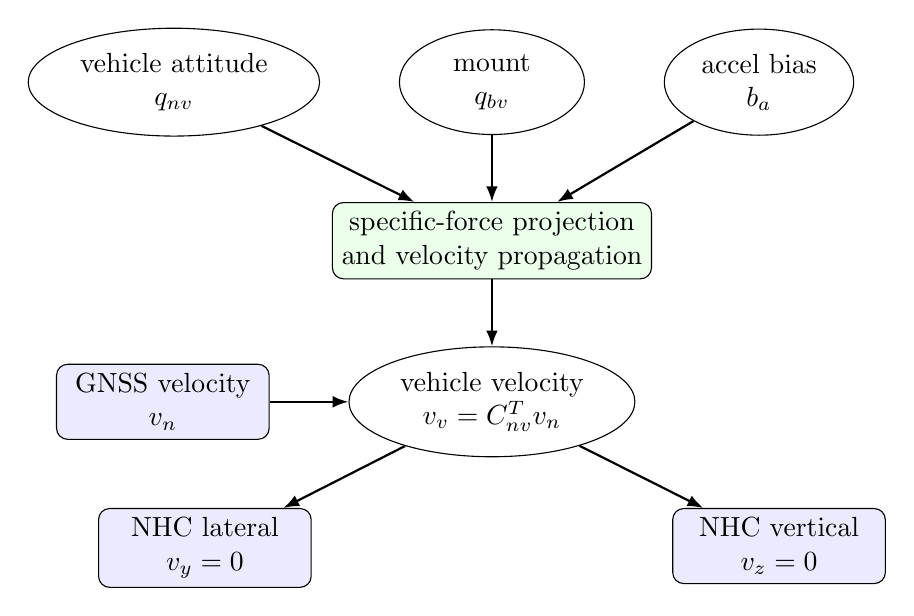
\begin{tikzpicture}[
  node distance=0.85cm and 1.0cm,
  state/.style={draw,ellipse,align=center,minimum width=2.35cm,minimum height=0.72cm},
  meas/.style={draw,rounded corners,fill=blue!8,align=center,minimum width=2.7cm,minimum height=0.78cm},
  dyn/.style={draw,rounded corners,fill=green!8,align=center,minimum width=2.9cm,minimum height=0.78cm},
  arr/.style={-{Latex[length=2mm]},thick}
]
  \node[state] (att) {vehicle attitude\\\(q_{nv}\)};
  \node[state,right=of att] (mount) {mount\\\(q_{bv}\)};
  \node[state,right=of mount] (bias) {accel bias\\\(b_a\)};
  \node[dyn,below=of mount] (prop) {specific-force projection\\and velocity propagation};
  \node[state,below=of prop] (vel) {vehicle velocity\\\(v_v=C_{nv}\T v_n\)};
  \node[meas,left=of vel] (gnss) {GNSS velocity\\\(v_n\)};
  \node[meas,below left=of vel] (nhcy) {NHC lateral\\\(v_y=0\)};
  \node[meas,below right=of vel] (nhcz) {NHC vertical\\\(v_z=0\)};
  \draw[arr] (att) -- (prop);
  \draw[arr] (mount) -- (prop);
  \draw[arr] (bias) -- (prop);
  \draw[arr] (prop) -- (vel);
  \draw[arr] (gnss) -- (vel);
  \draw[arr] (vel) -- (nhcy);
  \draw[arr] (vel) -- (nhcz);
\end{tikzpicture}
\caption{Generic local EKF context. Attitude, mount, and accelerometer bias
affect velocity propagation. GNSS velocity and NHC then determine whether those
effects can be separated.}
\end{figure}

\section{Roll Channel}

\subsection{Roll-Only State}

Use the roll-only local error state
\begin{equation}
  x_r=
  \begin{bmatrix}
  \phiv & \rhom & \delta b_{ay} & \delta b_{az} & \delta v_y & \delta v_z
  \end{bmatrix}\T .
\end{equation}
Here \(\phiv\) is vehicle roll error, \(\rhom\) is vehicle-to-body mount roll
error, \(\delta b_{ay}\) and \(\delta b_{az}\) are lateral and vertical
accelerometer correction errors after local projection, and
\(\delta v_y,\delta v_z\) are vehicle-frame lateral and vertical velocity
errors.

\subsection{Roll Dynamics}

For small roll errors, and ignoring second-order yaw/pitch products, the
lateral and vertical velocity error dynamics are approximately
\begin{align}
  \delta \dot v_y &\approx g\phiv - g\rhom - \delta b_{ay} + w_y, \label{eq:roll-vy}\\
  \delta \dot v_z &\approx -a_y\rhom - \delta b_{az} + w_z . \label{eq:roll-vz}
\end{align}
The sign convention can flip with implementation details, but the structure is
the invariant point: the lateral channel observes the difference between
vehicle roll and mount roll, while the vertical channel contains a mount-only
term proportional to lateral acceleration \(a_y\).

\begin{figure}[h]
\centering
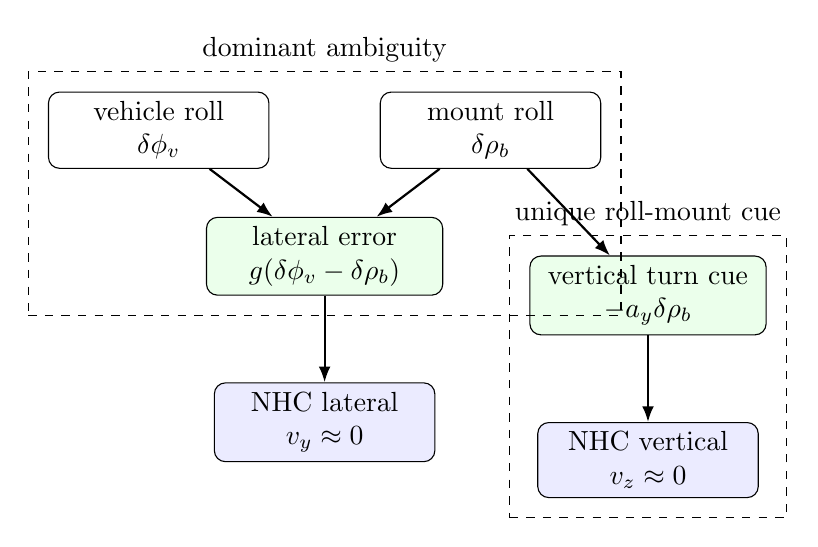
\begin{tikzpicture}[
  node distance=1.1cm and 1.4cm,
  block/.style={draw,rounded corners,align=center,minimum width=2.8cm,minimum height=0.8cm},
  obs/.style={draw,rounded corners,fill=blue!8,align=center,minimum width=2.8cm,minimum height=0.8cm},
  cue/.style={draw,rounded corners,fill=green!8,align=center,minimum width=3.0cm,minimum height=0.8cm},
  arr/.style={-{Latex[length=2mm]},thick}
]
  \node[block] (att) {vehicle roll\\\(\phiv\)};
  \node[block,right=of att] (mount) {mount roll\\\(\rhom\)};
  \node[cue,below=of $(att)!0.5!(mount)$] (latdyn) {lateral error\\\(g(\phiv-\rhom)\)};
  \node[cue,below=of mount,xshift=2.0cm] (vertdyn) {vertical turn cue\\\(-a_y\rhom\)};
  \node[obs,below=of latdyn] (nhcy) {NHC lateral\\\(v_y\approx0\)};
  \node[obs,below=of vertdyn] (nhcz) {NHC vertical\\\(v_z\approx0\)};
  \draw[arr] (att) -- (latdyn);
  \draw[arr] (mount) -- (latdyn);
  \draw[arr] (mount) -- (vertdyn);
  \draw[arr] (latdyn) -- (nhcy);
  \draw[arr] (vertdyn) -- (nhcz);
  \node[draw,dashed,fit=(att)(mount)(latdyn),inner sep=0.25cm,
        label={[align=center]above:dominant ambiguity}] {};
  \node[draw,dashed,fit=(vertdyn)(nhcz),inner sep=0.25cm,
        label={[align=center]above:unique roll-mount cue}] {};
\end{tikzpicture}
\caption{Roll ambiguity. The strongest roll signal is lateral gravity
projection, but it sees \(\phiv-\rhom\). The unique mount-roll cue enters
through vertical NHC during turns.}
\end{figure}

\subsection{Roll NHC Rows}

Over one short interval \(\dt\), Equations~\eqref{eq:roll-vy} and
\eqref{eq:roll-vz} give
\begin{align}
  r_y &\approx
    -\delta v_y-\dt(g\phiv-g\rhom-\delta b_{ay})+\eta_y,\\
  r_z &\approx
    -\delta v_z-\dt(-a_y\rhom-\delta b_{az})+\eta_z.
\end{align}
The corresponding Jacobian rows are
\begin{align}
  H_y &\approx
    \begin{bmatrix}
    -g\dt & +g\dt & +\dt & 0 & -1 & 0
    \end{bmatrix},\\
  H_z &\approx
    \begin{bmatrix}
    0 & +a_y\dt & 0 & +\dt & 0 & -1
    \end{bmatrix}.
\end{align}
Thus lateral NHC is strong but ambiguous. Vertical NHC is weaker but separates
mount roll from vehicle roll when \(a_y\) is nonzero.

\section{Pitch Channel}

\subsection{Pitch-Only State}

Use the pitch-only local error state
\begin{equation}
  x_p=
  \begin{bmatrix}
  \thetav & \pim & \delta b_{ax} & \delta b_{az} & \delta v_x & \delta v_z
  \end{bmatrix}\T .
\end{equation}
Here \(\thetav\) is vehicle pitch error, \(\pim\) is vehicle-to-body mount pitch
error, \(\delta b_{ax}\) and \(\delta b_{az}\) are longitudinal and vertical
accelerometer correction errors after local projection, and
\(\delta v_x,\delta v_z\) are vehicle-frame longitudinal and vertical velocity
errors.

\subsection{Pitch Dynamics}

For small pitch errors, the longitudinal and vertical velocity error dynamics
are approximately
\begin{align}
  \delta \dot v_x &\approx -g\thetav + g\pim - \delta b_{ax} + w_x, \label{eq:pitch-vx}\\
  \delta \dot v_z &\approx +a_x\pim - \delta b_{az} + w_z . \label{eq:pitch-vz}
\end{align}
The first row is the pitch analogue of the roll lateral row: it mainly observes
the difference between vehicle pitch and mount pitch. The second row is the
unique mount-pitch cue. It is driven by longitudinal acceleration \(a_x\), so
acceleration and braking maneuvers provide the excitation that separates mount
pitch from vehicle pitch.

\begin{figure}[h]
\centering
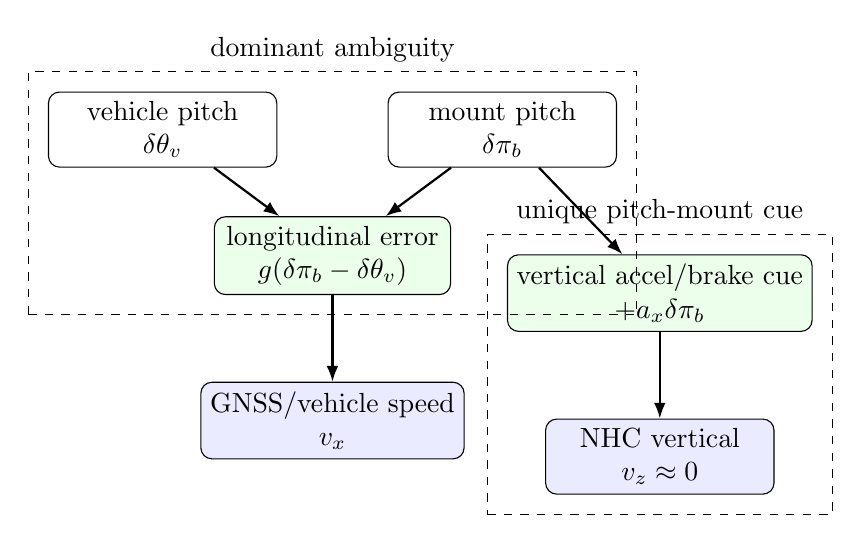
\begin{tikzpicture}[
  node distance=1.1cm and 1.4cm,
  block/.style={draw,rounded corners,align=center,minimum width=2.9cm,minimum height=0.8cm},
  obs/.style={draw,rounded corners,fill=blue!8,align=center,minimum width=2.9cm,minimum height=0.8cm},
  cue/.style={draw,rounded corners,fill=green!8,align=center,minimum width=3.0cm,minimum height=0.8cm},
  arr/.style={-{Latex[length=2mm]},thick}
]
  \node[block] (att) {vehicle pitch\\\(\thetav\)};
  \node[block,right=of att] (mount) {mount pitch\\\(\pim\)};
  \node[cue,below=of $(att)!0.5!(mount)$] (longdyn) {longitudinal error\\\(g(\pim-\thetav)\)};
  \node[cue,below=of mount,xshift=2.0cm] (vertdyn) {vertical accel/brake cue\\\(+a_x\pim\)};
  \node[obs,below=of longdyn] (speed) {GNSS/vehicle speed\\\(v_x\)};
  \node[obs,below=of vertdyn] (nhcz) {NHC vertical\\\(v_z\approx0\)};
  \draw[arr] (att) -- (longdyn);
  \draw[arr] (mount) -- (longdyn);
  \draw[arr] (mount) -- (vertdyn);
  \draw[arr] (longdyn) -- (speed);
  \draw[arr] (vertdyn) -- (nhcz);
  \node[draw,dashed,fit=(att)(mount)(longdyn),inner sep=0.25cm,
        label={[align=center]above:dominant ambiguity}] {};
  \node[draw,dashed,fit=(vertdyn)(nhcz),inner sep=0.25cm,
        label={[align=center]above:unique pitch-mount cue}] {};
\end{tikzpicture}
\caption{Pitch ambiguity. Vehicle pitch and mount pitch trade through
longitudinal gravity projection. Mount pitch becomes uniquely observable when
longitudinal acceleration or braking excites the vertical channel.}
\end{figure}

\subsection{Pitch Measurement Rows}

There is no ordinary NHC constraint on longitudinal velocity, because \(v_x\)
is the intended vehicle motion. Longitudinal velocity must therefore be
anchored by GNSS velocity, an optional vehicle-speed measurement, or the
integrated trajectory. A short-interval longitudinal velocity residual is
\begin{equation}
  r_x \approx
    -\delta v_x-\dt(-g\thetav+g\pim-\delta b_{ax})+\eta_x.
\end{equation}
The vertical NHC row is
\begin{equation}
  r_z \approx
    -\delta v_z-\dt(a_x\pim-\delta b_{az})+\eta_z.
\end{equation}
With state order \(x_p=[\thetav,\pim,\delta b_{ax},\delta b_{az},
\delta v_x,\delta v_z]\T\), the rows are
\begin{align}
  H_x &\approx
    \begin{bmatrix}
    +g\dt & -g\dt & +\dt & 0 & -1 & 0
    \end{bmatrix},\\
  H_z &\approx
    \begin{bmatrix}
    0 & -a_x\dt & 0 & +\dt & 0 & -1
    \end{bmatrix}.
\end{align}
The pitch analogue of roll's lateral NHC row is the longitudinal velocity row.
It is not a zero-velocity pseudo-measurement; it comes from GNSS velocity,
vehicle speed, or velocity consistency. The unique pitch-mount information is
again the vertical NHC row, now scaled by \(a_x\).

\section{Information Strength}

For roll, the approximate ratio of unique mount-roll information to coupled
roll information is
\begin{equation}
  \frac{I_{\rho,\text{unique}}}{I_{\rho,\text{coupled}}}
  \approx
  \frac{a_y^2/R_z}{g^2/R_y}
  =
  \left(\frac{a_y}{g}\right)^2\frac{R_y}{R_z}.
  \label{eq:roll-ratio}
\end{equation}
For pitch, the analogous ratio is
\begin{equation}
  \frac{I_{\pi,\text{unique}}}{I_{\pi,\text{coupled}}}
  \approx
  \frac{a_x^2/R_z}{g^2/R_x}
  =
  \left(\frac{a_x}{g}\right)^2\frac{R_x}{R_z},
  \label{eq:pitch-ratio}
\end{equation}
where \(R_x\) is the effective longitudinal velocity observation variance from
GNSS, vehicle speed, or the relevant batch update. If the longitudinal velocity
anchor is weak, pitch can still trade with mount pitch even when \(R_z\) is
tight.

Using representative NHC values \(R_y=0.5\), \(R_z=0.5\), the roll ratio is
\begin{equation}
  \left(\frac{a_y}{9.80665}\right)^2 .
\end{equation}
The same scale applies to pitch if \(R_x\approx R_y\). In practice \(R_x\) is
often different because forward velocity is measured rather than constrained to
zero.

\begin{center}
\begin{tabular}{>{\centering\arraybackslash}p{0.18\linewidth}
                >{\centering\arraybackslash}p{0.16\linewidth}
                >{\centering\arraybackslash}p{0.24\linewidth}
                >{\raggedright\arraybackslash}p{0.24\linewidth}}
\toprule
Excitation [m/s\(^2\)] & Maneuver & Ratio with coupled/vertical \(R=10\) & Interpretation \\
\midrule
0.5 & mild & 0.026 & very weak unique cue \\
1.0 & moderate & 0.104 & weak unique cue \\
2.0 & strong & 0.416 & useful but still coupled \\
3.0 & very strong & 0.936 & comparable to coupled cue \\
\bottomrule
\end{tabular}
\end{center}

\begin{figure}[h]
\centering
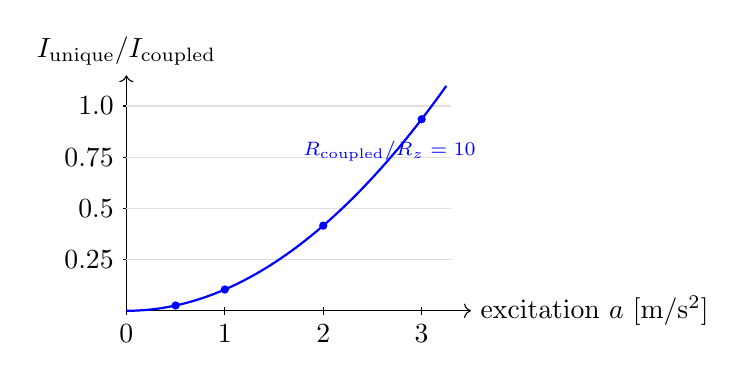
\begin{tikzpicture}[x=1.25cm,y=2.6cm]
  \draw[->] (0,0) -- (3.5,0) node[right] {excitation \(a\) [m/s\(^2\)]};
  \draw[->] (0,0) -- (0,1.15) node[above] {\(I_{\text{unique}}/I_{\text{coupled}}\)};
  \foreach \x/\lab in {0/0,1/1,2/2,3/3} {
    \draw (\x,0.02) -- (\x,-0.02) node[below] {\lab};
  }
  \foreach \y/\lab in {0.25/0.25,0.5/0.5,0.75/0.75,1/1.0} {
    \draw (0.03,\y) -- (-0.03,\y) node[left] {\lab};
    \draw[gray!25] (0,\y) -- (3.3,\y);
  }
  \draw[thick,blue,domain=0:3.25,samples=80]
    plot (\x,{10*(\x/9.80665)^2});
  \node[blue,anchor=west] at (1.7,0.78) {\scriptsize \(R_{\text{coupled}}/R_z=10\)};
  \fill[blue] (0.5,{10*(0.5/9.80665)^2}) circle (1.5pt);
  \fill[blue] (1.0,{10*(1.0/9.80665)^2}) circle (1.5pt);
  \fill[blue] (2.0,{10*(2.0/9.80665)^2}) circle (1.5pt);
  \fill[blue] (3.0,{10*(3.0/9.80665)^2}) circle (1.5pt);
\end{tikzpicture}
\caption{Unique mount-angle information is weak under mild excitation. Roll
uses lateral acceleration \(a_y\); pitch uses longitudinal acceleration
\(a_x\).}
\end{figure}

\section{Bias and Covariance Effects}

The ratios above are optimistic because they ignore bias. A one-degree
attitude or mount error projects gravity into a horizontal axis by
\begin{equation}
  g\sin(1^\circ)\approx0.171\ \text{m/s}^2 .
\end{equation}
The unique vertical cue from one degree of mount error during a
\(1\ \text{m/s}^2\) maneuver is only
\begin{equation}
  1.0\sin(1^\circ)\approx0.017\ \text{m/s}^2 .
\end{equation}
That term is an order of magnitude smaller. It can be absorbed by vertical
accelerometer bias or vertical velocity unless covariance and process noise
prevent those nuisance states from explaining persistent maneuver-correlated
residuals.

For a linearized update with information matrix
\begin{equation}
  \Lambda=H\T R^{-1}H,
\end{equation}
the information in a mount angle \(\alpha\) after marginalizing nuisance states
\(\xi\) is the Schur complement
\begin{equation}
  \Lambda_{\alpha|\xi}
  =
  \Lambda_{\alpha\alpha}
  -
  \Lambda_{\alpha\xi}\Lambda_{\xi\xi}^{-1}\Lambda_{\xi\alpha}.
  \label{eq:schur}
\end{equation}
For roll,
\begin{equation}
  \alpha=\rhom,\qquad
  \xi=
  \begin{bmatrix}
  \phiv & \delta b_{ay} & \delta b_{az} & \delta v_y & \delta v_z
  \end{bmatrix}\T .
\end{equation}
For pitch,
\begin{equation}
  \alpha=\pim,\qquad
  \xi=
  \begin{bmatrix}
  \thetav & \delta b_{ax} & \delta b_{az} & \delta v_x & \delta v_z
  \end{bmatrix}\T .
\end{equation}
This is the clean quantitative measure of whether the data window uniquely
informs the mount angle after attitude, velocity, and bias are allowed to
absorb the same residual.

\section{Implications}

\begin{enumerate}[leftmargin=*]
  \item Vehicle roll and mount roll are nearly interchangeable in the lateral
        channel. They are separated mainly by vertical NHC during lateral
        acceleration.
  \item Vehicle pitch and mount pitch are nearly interchangeable in the
        longitudinal channel. They are separated mainly by vertical NHC during
        acceleration and braking.
  \item GNSS velocity is necessary because it prevents \(v_y\), \(v_z\), and
        \(v_x\) from becoming hidden residual reservoirs, but it does not by
        itself make mount and vehicle attitude unique.
  \item Bias covariance matters because the unique vertical cue is small. If
        vertical accelerometer bias is too flexible, it can absorb the same
        residual that should correct mount.
  \item Mount covariance must remain flexible until enough uniquely informative
        excitation has accumulated. Premature covariance collapse makes the
        filter retain an incorrect roll/pitch split.
\end{enumerate}

\section{Recommended Replay Diagnostic}

For each replay window, compute the linearized rows for NHC and velocity
observations in the local EKF basis and accumulate
\begin{equation}
  \Lambda_W=\sum_{k\in W} H_k\T R_k^{-1}H_k .
\end{equation}
Then report the raw and marginalized mount information:
\begin{align}
  I_{\alpha,\text{raw}} &= \Lambda_{\alpha\alpha},\\
  I_{\alpha|\beta} &=
    \Lambda_{\alpha\alpha}
    -\Lambda_{\alpha\beta}\Lambda_{\beta\beta}^{-1}\Lambda_{\beta\alpha},\\
  I_{\alpha|\xi} &=
    \Lambda_{\alpha\alpha}
    -\Lambda_{\alpha\xi}\Lambda_{\xi\xi}^{-1}\Lambda_{\xi\alpha}.
\end{align}
For roll, \(\alpha=\rhom\) and \(\beta=\phiv\). For pitch,
\(\alpha=\pim\) and \(\beta=\thetav\). The raw value shows apparent mount
information. The second value removes the vehicle-attitude ambiguity. The
third value removes attitude, velocity, and accelerometer-bias nuisance states
and is the most useful scalar observability metric.

\section{Implemented Synthetic Experiment}

The repository includes a repeatable diagnostic that exercises this theory in
the local NED convention:
\begin{verbatim}
cargo run --release -p sim --bin diag_mount_observability
\end{verbatim}
The diagnostic generates truth-noise synthetic scenarios with the same injected
initial mount error, computes the Schur-complement information proxies above,
and then runs the EKF with two covariance splits:
\begin{itemize}[nosep]
  \item \texttt{qerr\_mount\_flex}: tighter vehicle-attitude covariance and
        looser mount covariance,
  \item \texttt{qerr\_att\_flex}: looser vehicle-attitude covariance and
        tighter mount covariance.
\end{itemize}
If the data do not uniquely separate vehicle attitude from mount attitude, the
final mount estimate depends strongly on this covariance split. That covariance
sensitivity is itself evidence of weak observability. If a maneuver provides
strong unique excitation, the Schur-complement information should increase for
the corresponding axis: lateral acceleration for roll, and longitudinal
acceleration/braking for pitch.

\end{document}
